\documentclass[12pt]{article}
\usepackage[utf8]{inputenc}
\usepackage[left=2cm,right=2cm,top=2cm,bottom=2cm]{geometry}
\usepackage[spanish]{babel}
\usepackage{graphicx, amsmath, multirow}
\usepackage[small]{caption}
\usepackage{subcaption}
\usepackage{url}
\setlength{\parskip}{\baselineskip}
\graphicspath{ {images/} }

\spanishdecimal{.}
\usepackage{hyperref}
\hypersetup{
	colorlinks=true,
	linkcolor=blue,     
	urlcolor=blue,
	citecolor=blue,
}


\begin{document}

	\thispagestyle{empty}

	\begin{center}
		{\Large \bf Valor esperado y varianza}\\
		Gabriela S\'anchez Y.\\
		5064
	\end{center}
  
  	En la presente actividad se simulan problemas previamente que previamente se resolvieron de forma analítica \cite{mpa_gabyt9}, con el objetivo de encontrar evidencia numérica que apoye el resultado analítico. Las simulaciones se realizan con el apoyo del lenguaje de programación \textsc{R} \cite{rstatistics}. El código puede consultarse en el archivo \texttt{t10.R} \cite{mpa_gaby}.
	
	{\bf Ejercicio 1, página 247}
	
	{\em A card is drawn at random from a deck consisting of cards numbered $2$ through $10$. A player wins $1$ dollar if the number on the card is odd and loses $1$ dollar if the number if even. What is the expected value of his winnings?}
	
	El resultado analítico de este problema es $-\frac{1}{9}$. Como primera aproximación para apoyar dicho resultado se realizan dos simulaciones del juego, en cada una se guarda la frecuencia y la frecuencia relativa con que cada resultado ocurre, además se calcula el promedio de las ganancias. En el cuadro \ref{table_outcomes} se pueden observar estos resultados. 
	
	\begin{table}[h]
		\caption{Frecuencias para el juego de las cartas.}
		\label{table_outcomes}
		\centering
		\begin{tabular}{|r|c|c|c|c|}
			\hline
			\multirow{3}{*}{\bf Ganancia} & \multicolumn{2}{c|}{\bf $n=100$} & \multicolumn{2}{c|}{\bf $n=10,000$} \\
			\cline{2-5}
			& \multirow{2}{*}{\bf Frecuencia} & \bf Frecuencia  &  \multirow{2}{*}{\bf Frecuencia} & \bf Frecuencia\\
			& & \bf relativa & & \bf relativa \\
			\hline
			-1 & 54 & 0.54 & 5578 & 0.5578 \\
			1 & 46 & 0.46 & 4422 & 0.4422 \\
			\hline
			\bf Ganancia promedio & \multicolumn{2}{r|}{\bf -0.08} & \multicolumn{2}{r|}{\bf -0.1156} \\
			\hline
		\end{tabular}
	\end{table}
	
	La ganancia promedio al jugar cien veces es de -0.08 y al jugar 10,000 veces de -0.1156. Se puede observar que este último resultado concuerda un poco mejor con el valor esperado de la ganancia.

	Es claro que estos resultados pueden variar, por lo que se realizan réplicas del juego para observar cómo varía la ganancia promedio. Los resultados obtenidos para cien réplicas se muestran en la figura \ref{hist_cartas}. La ganancia promedio se encuentra en su mayoría entre -0.1 y -0.2 cuando se juega cien veces y, entre -0.12 y -0.10 cuando se juega 10,000 veces. Es decir, los resultados se acercan al valor real.
	
	\begin{figure}
		\begin{subfigure}{0.5\textwidth}
			\centering
			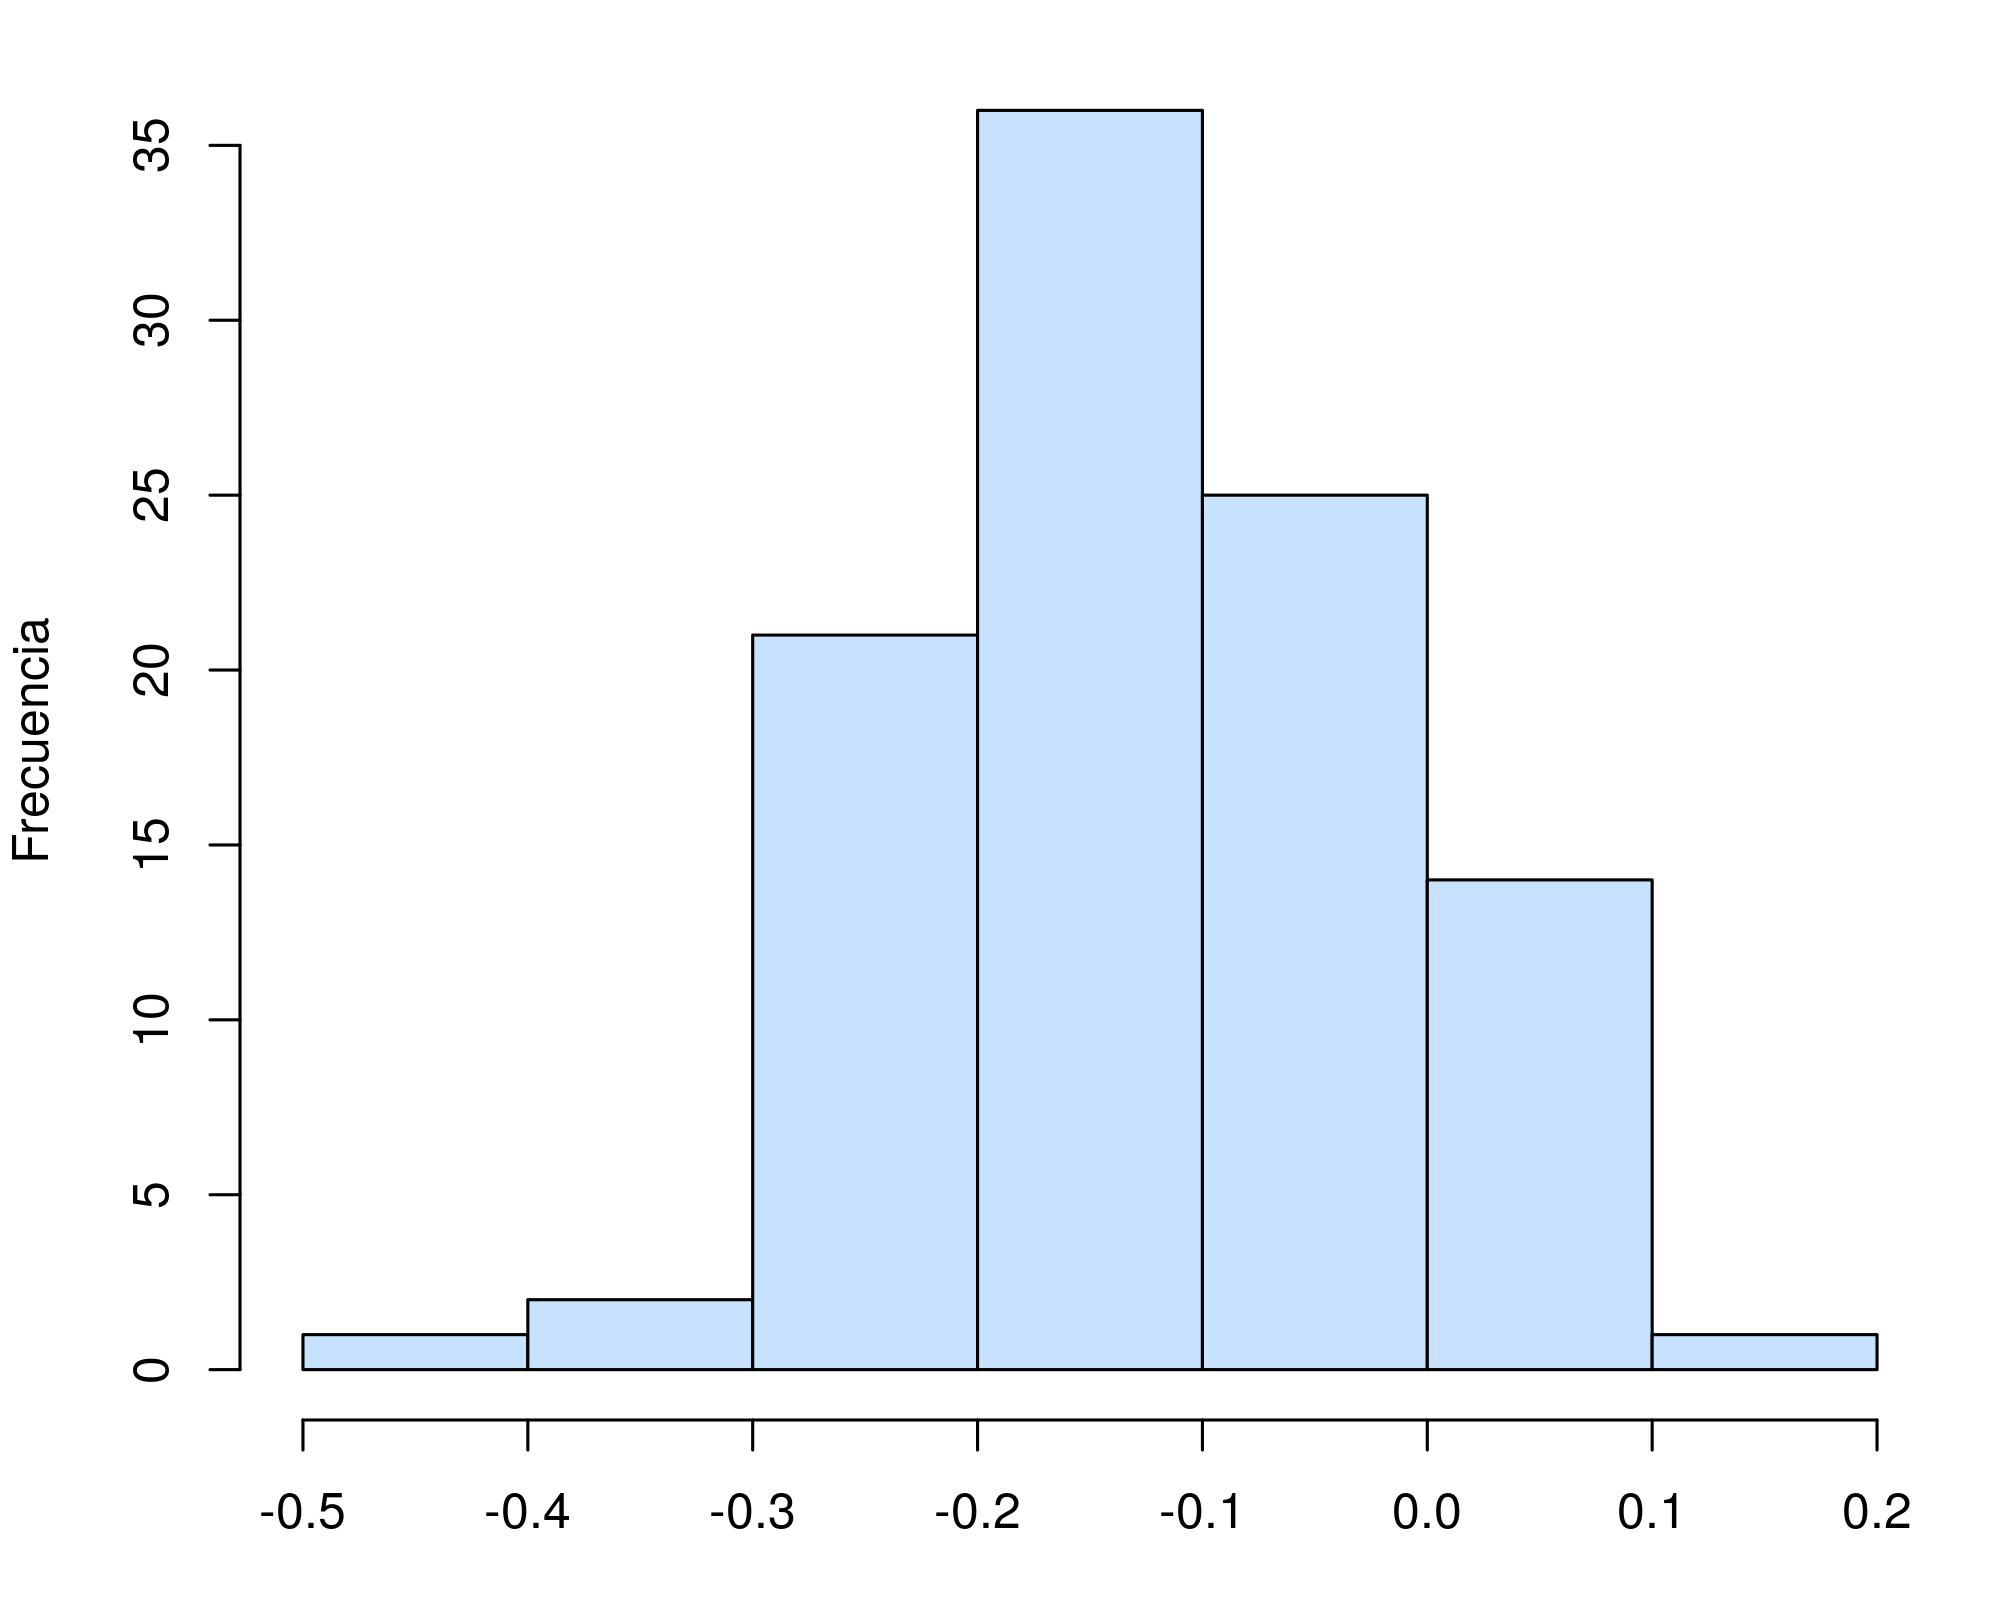
\includegraphics[scale=0.5]{juego_cartas1.png}
			\caption{$n=100$}
		\end{subfigure}
		\begin{subfigure}{0.5\textwidth}
		\centering
		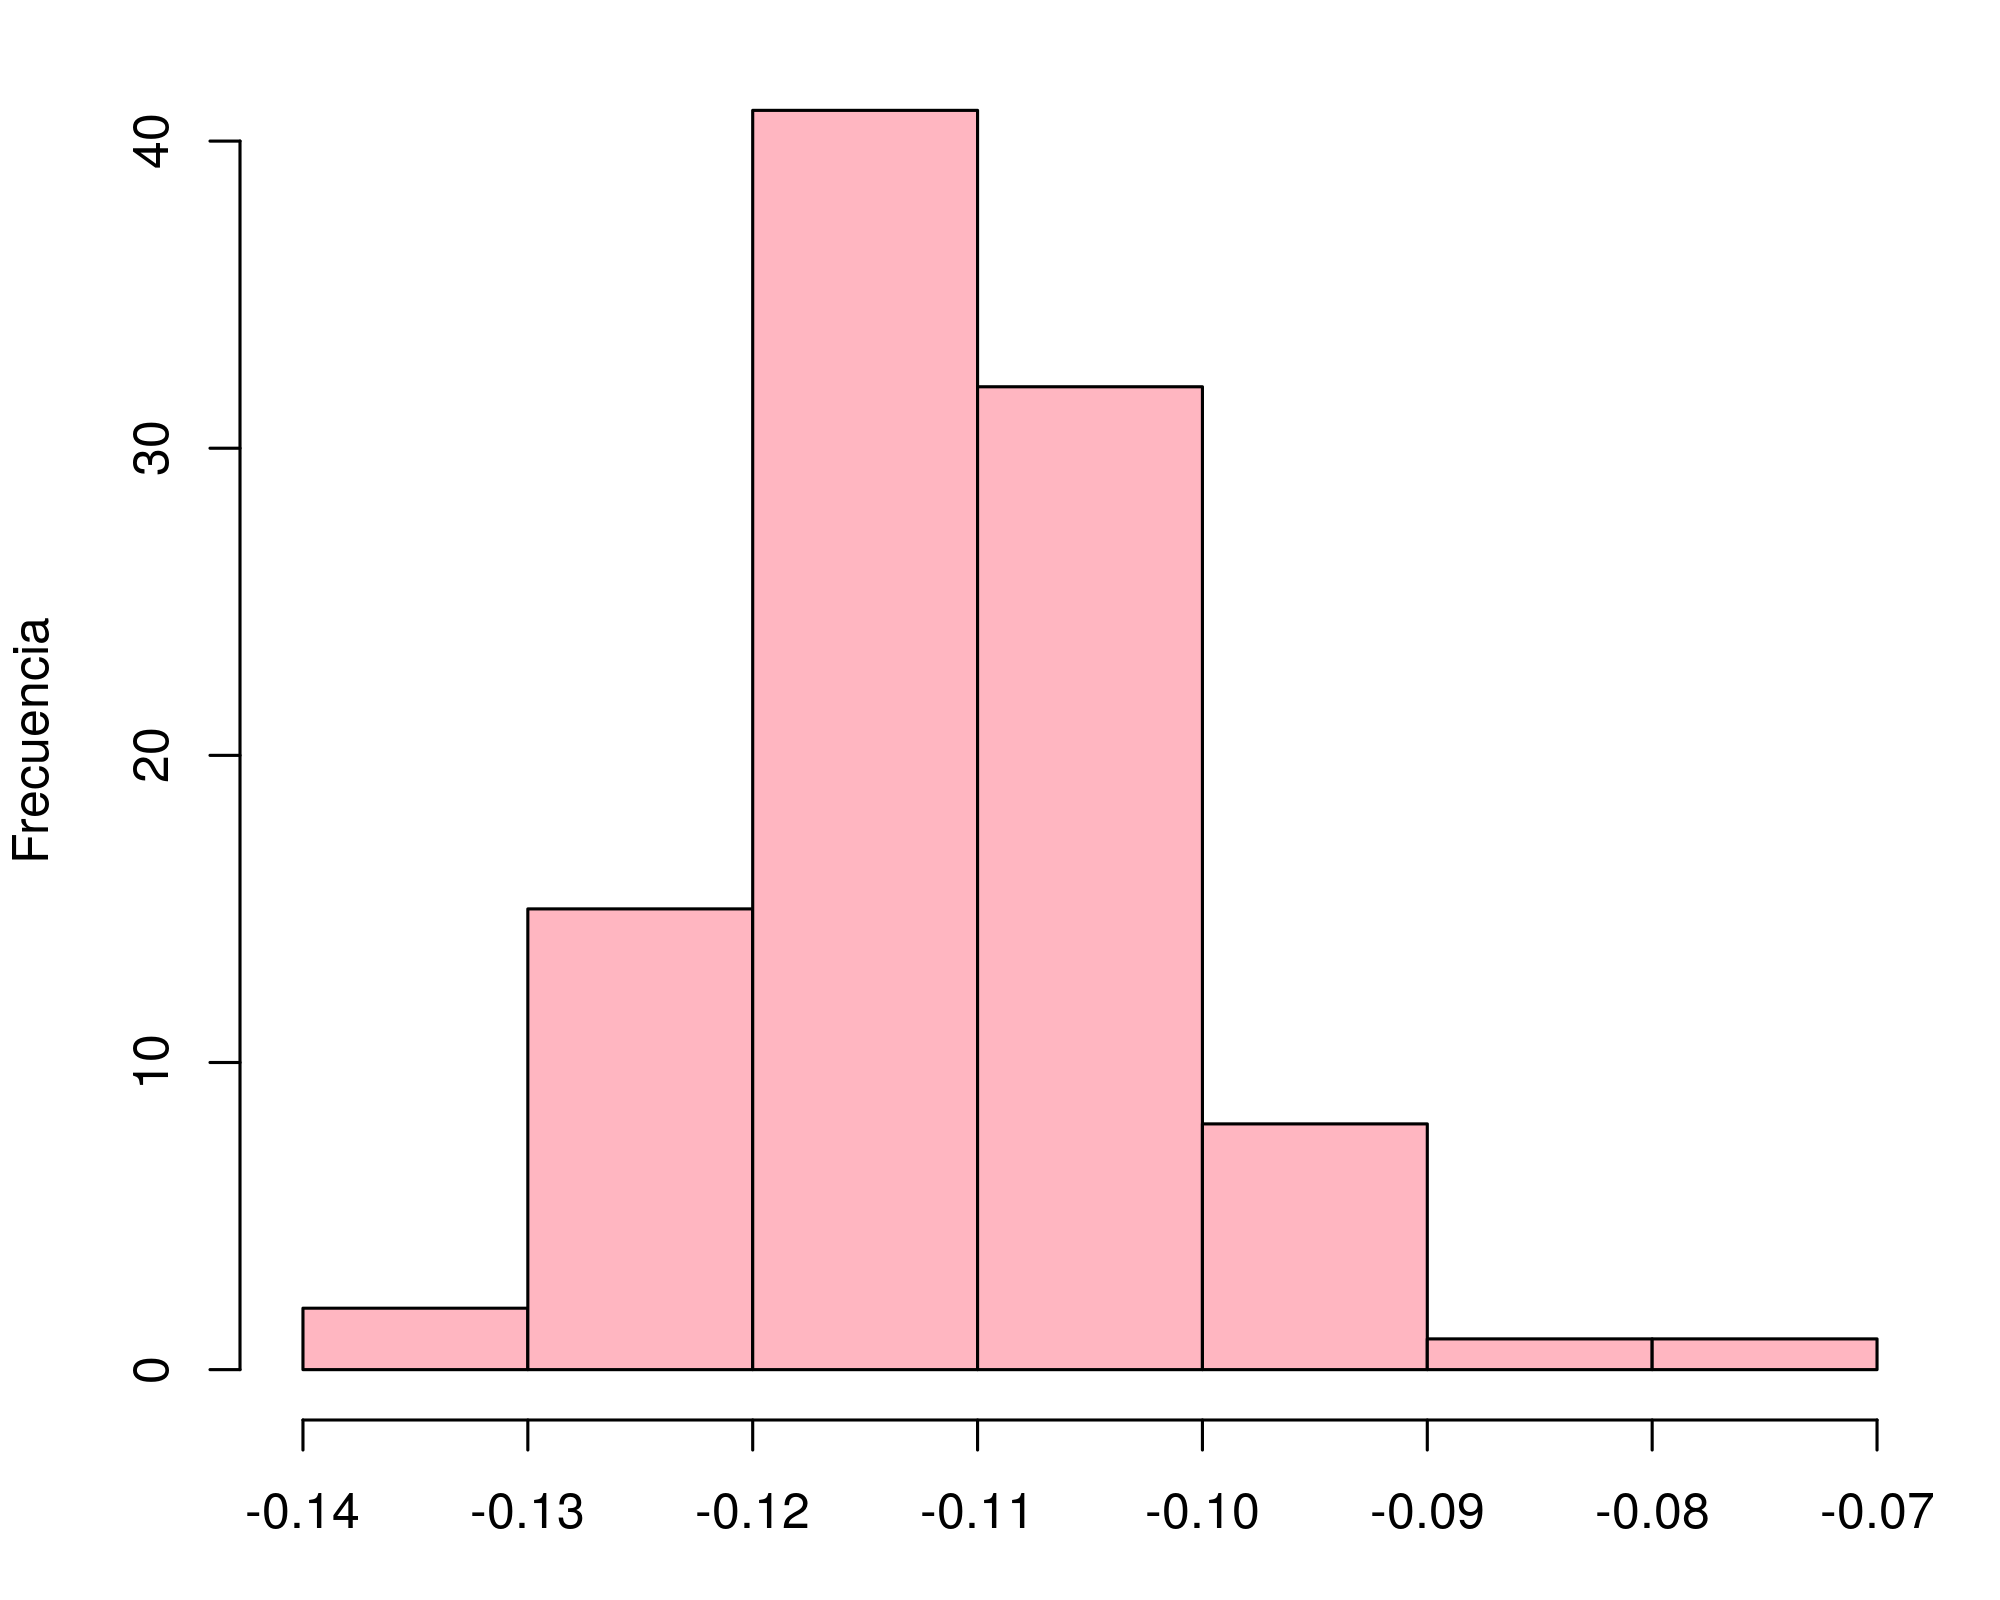
\includegraphics[scale=0.5]{juego_cartas2.png}
		\caption{$n=10,000$}
	\end{subfigure}
	\caption{Ganancia promedio del juego de cartas.}
	\label{hist_cartas}
	\end{figure}
	
%	
%	{\bf Excercise 6, page 247}
%	
%	{\em A die is rolled twice. Let $X$ denote the sum of the two numbers that turn up, and Y the difference of the numbers (specifically, the number on the first roll minus the number on the second). Show that $E[XY] = E[X]E[Y]$. Are $X$ and $Y$ independent?}
	
	
	{\bf Ejercicio 15, página 249}
	
	{\em A box contains two gold balls and three silver balls. You are allowed to choose successively balls from the box at random. You win 1 dollar each time you draw a gold ball and lose 1 dollar each time you draw a silver ball. After a draw, the ball is not replaced. Show that, if you draw until you are ahead by 1 dollar or until there are no more gold balls, this is a favorable game.}
	
	Previamente se determinó que el valor esperado jugando con las condiciones indicadas es $0.2$. El experimento diseñado para apoyar ese resultado es el siguiente: se plantea un experimento donde se juega cien veces. Ya que la elección es al azar, un sólo resultado del experimento no aporta mucha información por lo que se realizan cien réplicas. Los resultados obtenidos de la ganancia promedio se muestran en el diagrama de caja bigote de la figura \ref{pelotas}. Note que la media de las ganancias obtenidas en las distintas réplicas es muy cercana a 0.2, de esta forma se tiene evidencia numérica que respalda el resultado obtenido previamente.
	
	\begin{figure}
		\centering
		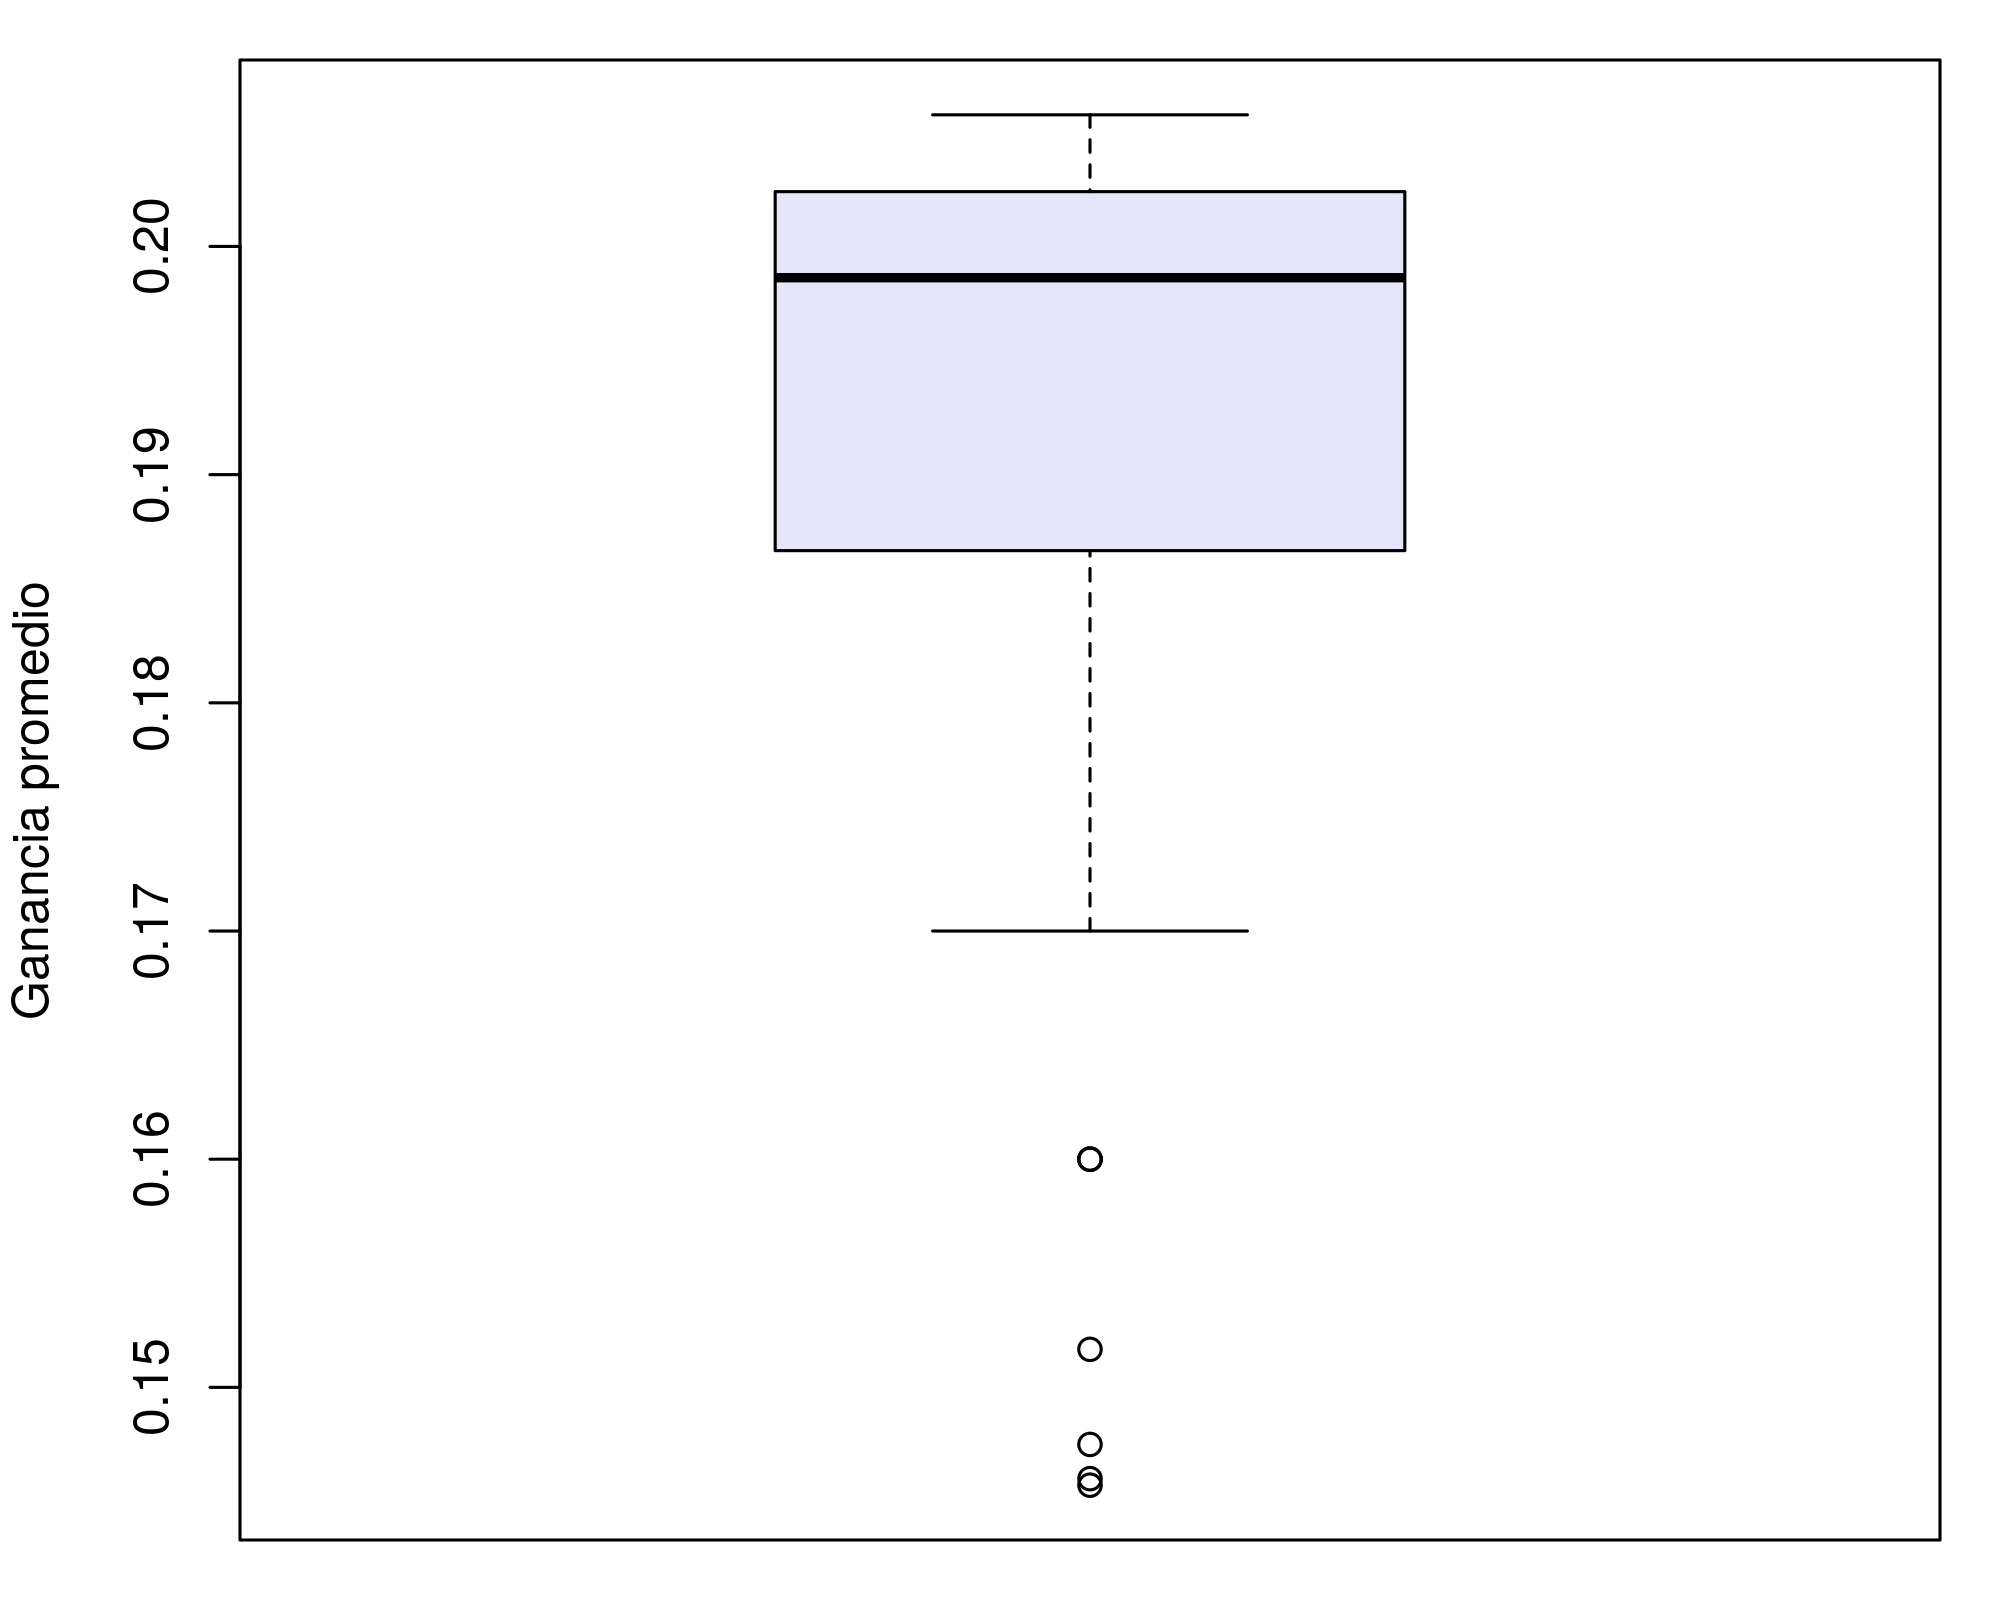
\includegraphics[scale=0.5]{pelotas.png}
		\caption{Diagrama de caja bigote de las ganancias obtenidas en cien réplicas del experimento.}
		\label{pelotas}
	\end{figure}
	
	%Es claro que si se jugara el juego sin las condiciones indicadas, no sería favorable ya que hay más pelotas plateadas que doradas pero 
	Es interesante analizar qué tanto cambia el valor esperado al modificar las condiciones de juego. Suponga que ahora el jugador se retira cuando lleva una ventaja de 1 dólar o luego de sacar dos pelotas, ¿cuál es el valor esperado de las ganancias en este caso?. 
	
	Jugar con esas condiciones reduce el espacio muestral a tres casos: $G$, $SG$ y $SS$, cada uno con probabilidad 2/5, 3/10 y 3/10, respectivamente; donde $G$ representa una pelota dorada y $S$ una plata. El valor esperado es $E[X] = 1(2/5) + 0(3/20) - 2(3/10) = -1/5$.
	
	Para responder a esta pregunta de forma numérica, se plantea el mismo experimento realizado previamente con la única diferencia de las condiciones de paro en el juego. Los resultados de la ganancia promedio se muestran en el diagrama de caja bigote de la figura \ref{pelotas_gana1_osale2}. Se puede concluir que el juego ha dejado de ser favorable, ahora la media de las ganancias es muy cercana a -0.2. Nótese que el resultado se aproxima al analítico que se ha calculado anteriormente.%la media de las ganancias obtenidas también es muy 
	
	\begin{figure}
		\centering
		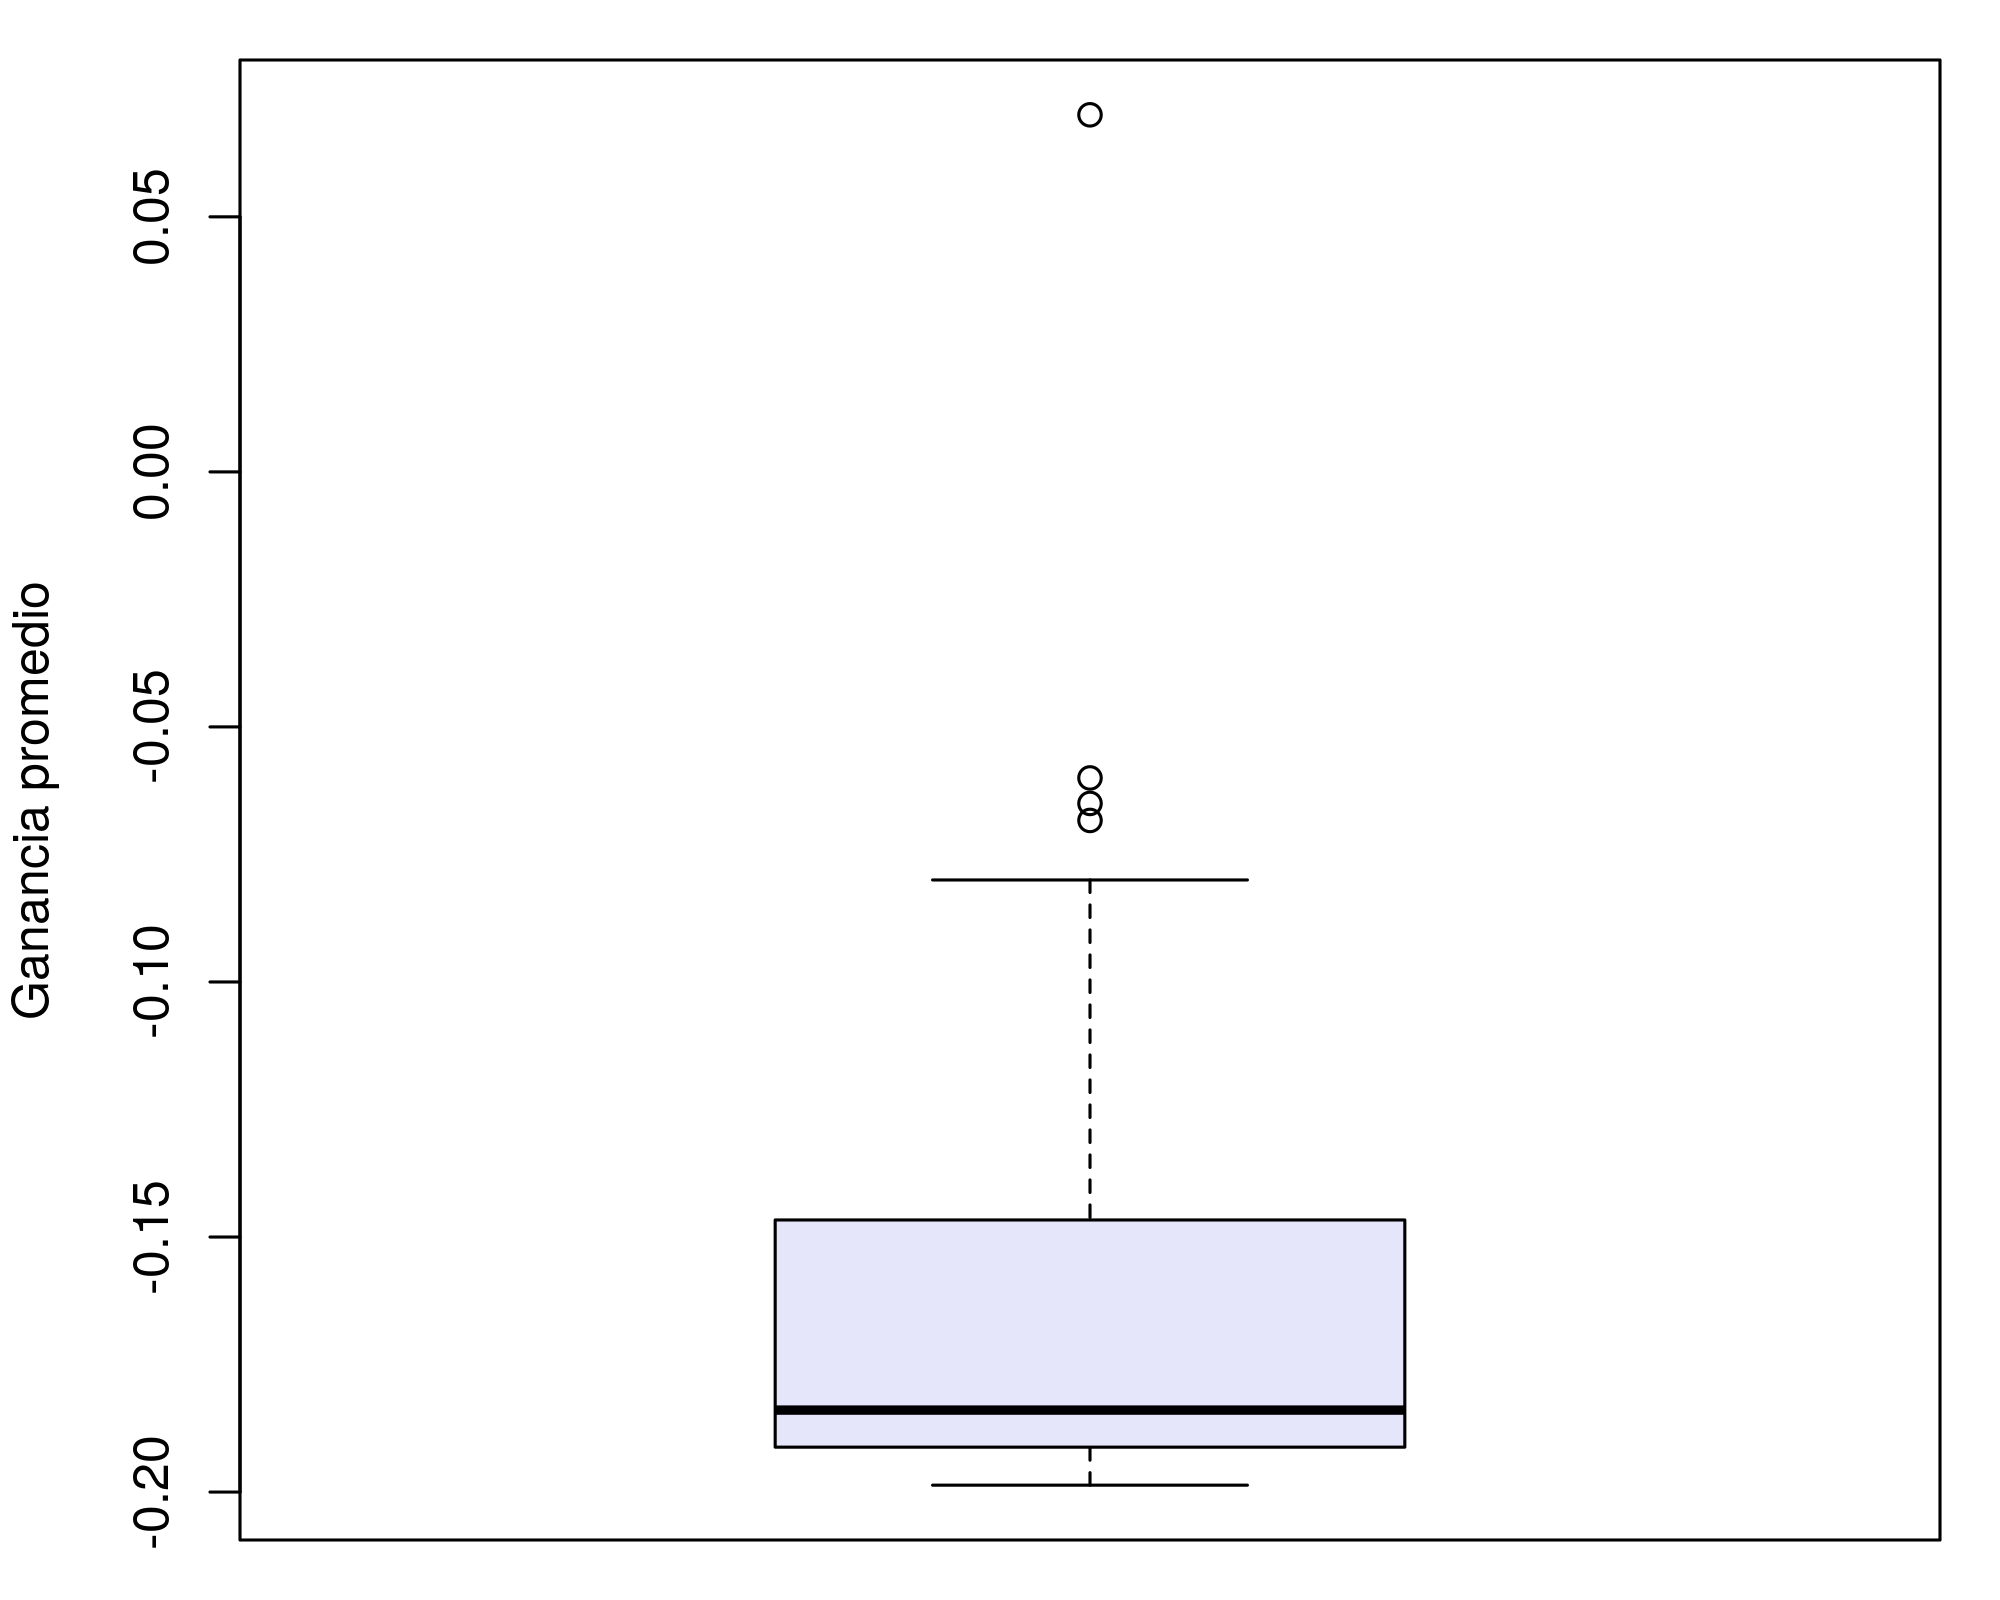
\includegraphics[scale=0.5]{pelotas_gana1_osale2.png}
		\caption{Ganancia promedio cuando el jugador se retira con una ventaja de 1 dólar o luego de sacar dos pelotas.}
		\label{pelotas_gana1_osale2}
	\end{figure}
	
	{\bf Ejercicio 18, página 249}
	
	{\em Exactly one of six similar keys opens a certain door. If you try the keys, one after another, what is the expected number of keys that you will have to try before success?}
	
	La simulación de este problema sigue un criterio similar al planteado para los ejercicios anteriores. El experimento consiste en realizar la prueba de las llaves hasta llegar a la correcta un total de cien veces y se replica 500. El promedio de los intentos fallidos antes de llegar al correcto obtenido en los experimentos se muestra en el diagrama de caja bigote de la figura \ref{keys}. La media de la simulación casi coincide con el valor analítico de 0.5.
	
	\begin{figure}
		\centering
		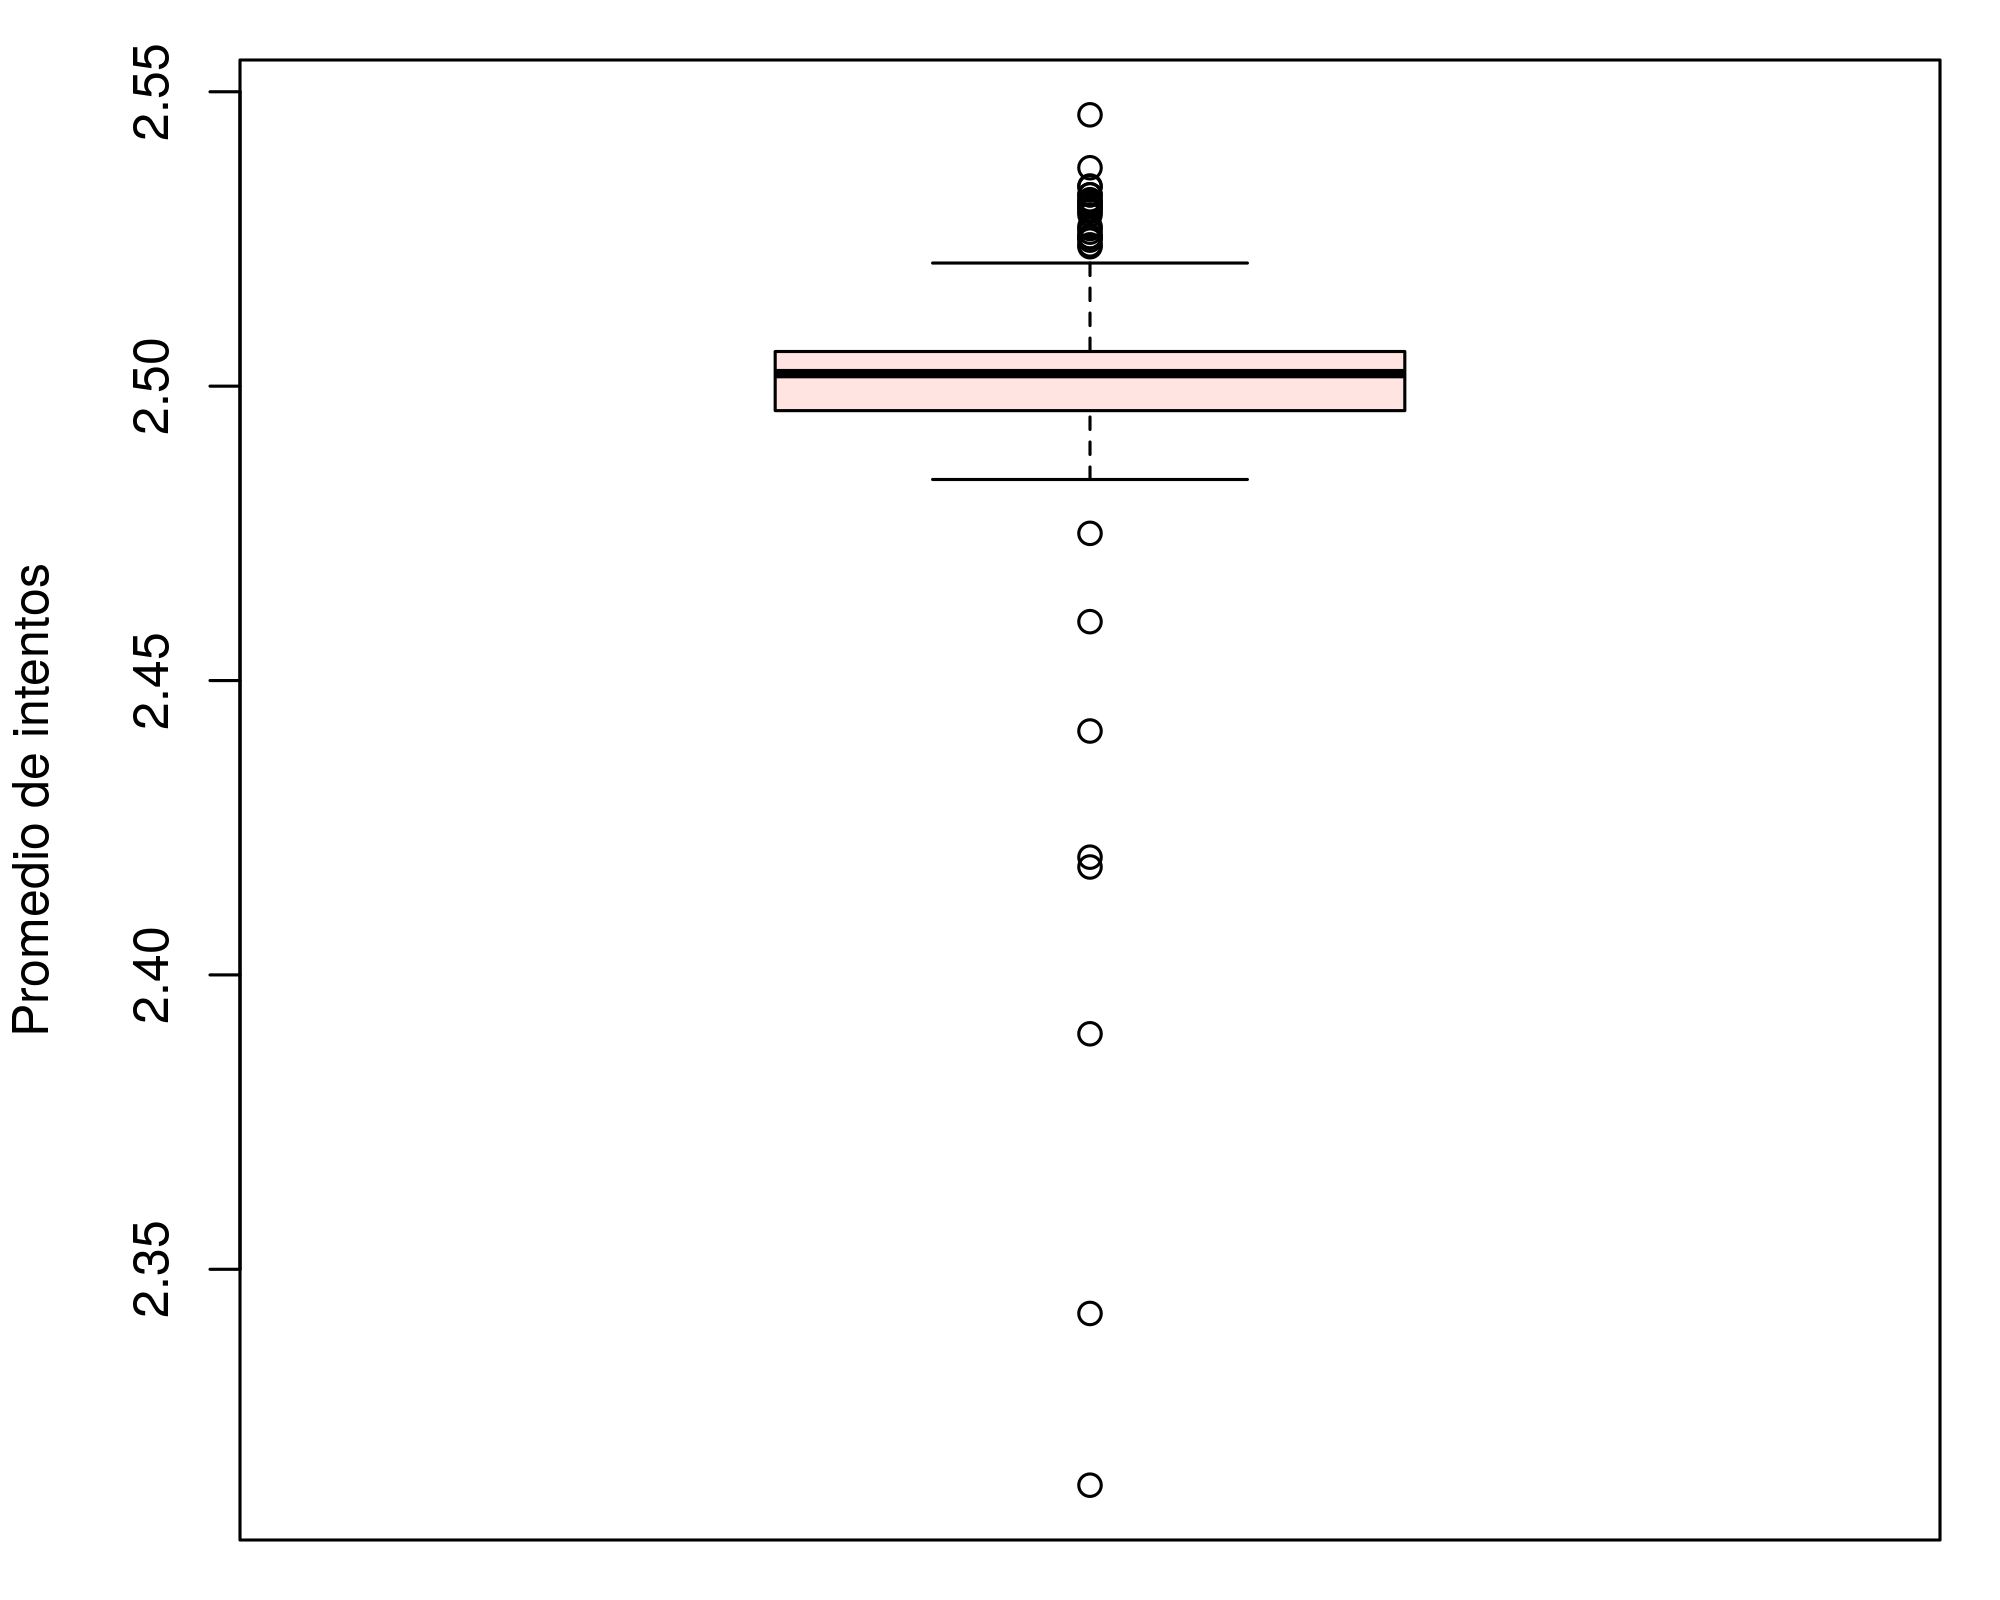
\includegraphics[scale=0.5]{llaves.png}
		\caption{Promedio de intentos fallidos antes de encontrar la llave correcta.}
		\label{keys}
	\end{figure}

%	{\bf Exercise 19, page 249}
%	
%	{\em A multiple choice exam is given. A problem has four possible answers, and exactly one answer is correct. The student is allowed to choose a subset of the four possible answers as his answer. If his chosen subset contains the correct answer, the student receives three points, but he loses one point for each wrong answer in his chosen subset. Show that if he just guesses a subset uniformly and randomly his expected score is zero.}
	
%	{\bf Ejercicio 3, página 278}
%	
%	{\em The lifetime, measure in hours, of the ACME super light bulb is a random variable T with density function \(f_T (t) = \lambda^2 te^{- \lambda t}\), where \(\lambda = 0.05\). What is the expected lifetime of this light bulb? What is its variance?}
	
	
	
	
\bibliographystyle{plain}
\bibliography{biblio}

\end{document}
